\section*{Uden hjælpemidler}
\begin{opgavetekst}{Opgave 1}
	Bestem følgende brøker
	\begin{align*}
		&1) \   \frac{3}{5} + \frac{9}{15}   &&2) \  \frac{7}{9}\cdot\frac{2}{3}     \\
		&3) \  \frac{\frac{1}{2}}{\frac{4}{10}}    &&4) \  2\cdot \frac{1}{4} + \frac{7}{6}    
	\end{align*}
\end{opgavetekst}

\begin{opgavetekst}{Opgave 2}
	Forkort følgende regneudtryk
	\begin{align*}
		&1) \   a^2\cdot a^5    &&2) \ \frac{b^9}{b^5}     \\
		&3) \   (c^2)^5    &&4) \  \left(\frac{d^7\cdot d^3}{d^2}\right)^3    
	\end{align*}
\end{opgavetekst}

\begin{opgavetekst}{Opgave 3}
\end{opgavetekst}

\begin{delopgave}{}{1}
	Bestem $10\%$ af 200.
\end{delopgave}
\begin{delopgave}{}{2}
	Forøg 50 med $20\%$.
\end{delopgave}
\begin{delopgave}{}{3}
	Bestem den procentvise forskel fra 50 til 70.
\end{delopgave}


\begin{opgavetekst}{Opgave 4}
	En eksponentialfunktion $f$ er givet ved
	\begin{align*}
		f(x) = 7.2\cdot 1.4^x
	\end{align*}
\end{opgavetekst}
\begin{delopgave}{}{1}
	Aflæs fremskrivningsfaktoren og begyndelsesværdien for $f$
\end{delopgave}
\begin{delopgave}{}{2}
	Bestem vækstraten for $f$.
\end{delopgave}

\begin{opgavetekst}{Opgave 5}
	På Figur \ref{fig:grafer} ses graferne $A,$ $B$ og $C$ for tre eksponentialfunktioner
	\begin{align*}
		f(x) &= 5\cdot 1.2^x,\\
		g(x) &= 6 \cdot 0.7^x,  \\
		h(x) &= 2 \cdot 1.4^x.
	\end{align*}
	\begin{figure}[H]
		\centering
		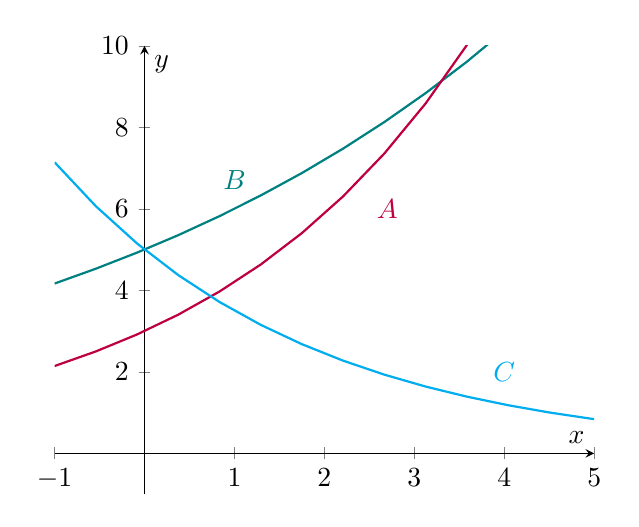
\begin{tikzpicture}
			\begin{axis}[
				axis lines = center,
				xmin = -1, xmax = 5,
				ymin = -1, ymax = 10,
				xlabel = $x$, ylabel = $y$]
				\addplot[thick, color = teal, domain = -1:10] {5*1.2^x};
				\addplot[thick, color = purple, domain = -1:10] {3*1.4^x};
				\addplot[thick, color = cyan, domain = -1:10] {5*0.7^x};
				\node[color = teal] at (axis cs: 1,6.7) {$B$};
				\node[color = purple] at (axis cs: 2.7,6) {$A$};
				\node[color = cyan] at (axis cs: 4,2) {$C$};
			\end{axis}
		\end{tikzpicture}	
		\caption{Graferne $A$, $B$ og $C$.}
		\label{fig:grafer}
	\end{figure}
	\phantom{h}
\end{opgavetekst}
\begin{delopgave}{}{1}
	Afgør hvilke af graferne $A$, $B$ og $C$ der tilhører funktionerne $f$, $g$ og $h$. Begrund dit svar.
\end{delopgave}


\newpage

\section*{Med hjælpemidler}

\begin{opgavetekst}{Opgave 6}
	Grafen for eksponentialfunktionen $f$ skærer gennem punkterne $(4,5)$ og $(6,22)$.
\end{opgavetekst}
\begin{delopgave}{}{1}
	Bestem forskriften for $f$. 
\end{delopgave}
\begin{delopgave}{}{2}
	Løs ligningen $f(x) = 30$. 
\end{delopgave}

\begin{opgavetekst}{Opgave 7}
	\begin{center}
		
\includegraphics[width= 0.6\textwidth]{Billeder/Bakterie}
	\end{center}
	Antallet af bakterier i Bakteriekoloni $\alpha$ er på 1250 bakterier. Antallet af bakterier vokser med 15 procent hvert døgn.
\end{opgavetekst}
\begin{delopgave}{}{1}
	Opstil en model, der beskriver antallet af bakterier i kolonien efter $x$ døgn. 
\end{delopgave}
\begin{delopgave}{}{2}
	Bestem antallet af bakterier efter 14 døgn. 
\end{delopgave}
\begin{meretekst}
	Bakteriekoloni $\beta$ har en bakterievækst, der kan beskrives ved funktionen
	\begin{align*}
		g(x) = 600\cdot 1.25^x,
	\end{align*}
	hvor $x$ er den passerede tid i døgn og $g$ er antal bakterier. 
\end{meretekst}
\begin{delopgave}{}{3}
	Tegn graferne for $f$ og $g$ i samme koordinatsystem.
\end{delopgave}

\begin{delopgave}{}{4}
	Bestem tidspunktet hvor antallet af bakterier i Bakteriekoloni $\beta$ overstiger antallet af bakterier i Bakteriekoloni $\alpha$ ved at løse en ligning. 
\end{delopgave}	

\begin{opgavetekst}{Opgave 8}
	\begin{center}
		\includegraphics[width=0.6\textwidth]{Billeder/alien}
	\end{center}
	På planeten Glorb, der er naboplanet til Flarp er sygdommen glub også brudt ud. Antallet af smittede kan ses af \href{https://github.com/ChristianJLex/TeachingNotes/raw/master/2023-2024/Data%20og%20lign/smittedeGlorb.xlsx}{\color{blue!60} dette regneark}. Det antages, at antal smittede Glorbere kan beskrives ved en funktion af typen
	\begin{align*}
		f(x) = b \cdot a^x,
	\end{align*}
	hvor $x$ er antal passerede dage og $f$ er antal smittede Glorbere.
\end{opgavetekst}
\begin{delopgave}{}{1}
	Lav regression på datasættet og bestem tallene $a$ og $b$.
\end{delopgave}
\begin{delopgave}{}{2}
	Hvor mange smittede Glorbere er der efter 50 dage i følge modellen?
\end{delopgave}
\begin{delopgave}{}{3}
	Hvornår overstiger antal smittede Glorbere 2 mio i følge modellen?
\end{delopgave}	
